\documentclass[journal]{IEEEtran}
\input{settings}
\begin{document}

\section{Alloyにおける時相論理の記述法の提案}
\label{sec:ProposedModel-TemporalLogic}
この章では、イベント発生時におけるウェブの様々な要素の状態変化の表現に利用可能なAlloyでの時相論理の記述法を提案する。

前述の\ref{sec:existing-models-problems}節における既存モデルの時相論理の表現能力の主な問題点は、「3状態以上の遷移を表現できない」ことである。
この問題は、Cookieモデルにおいて状態クラス(CookieモデルにけるCSStateクラス)間の関係性がHTTPTransactionクラスのみを用いて表現されていることに起因している。
この方式では同一のHTTPTransacion内の状態変化しか表現できない。
したがって、HTTPTransactionクラスに依存せずに、状態クラス間の関係性を表現する方式が必要となる。
また、CookieモデルにおけるCSStateはCookieの状態を表現するクラスであり、ウェブの他の要素を表現するための拡張性に乏しい。
そこで、拡張性を高めるため、様々なウェブの構成要素の状態を表現するための汎用的な状態クラスを定義し、その状態クラス間の関係性を表現することを目標とする。

本研究では各状態クラス間の状態遷移の表現のために必要な命題論理を、述語として容易に利用できる形式にまとめる。
ここで、時間軸全体を通した状態遷移を表現するためにどのような述語が必要となるかを考える。
まず、ある二状態に対してそれらが時間軸上で連続しているかを判定できれば、
「前後の二状態で起こりうる変化」を表現可能になる。
これに加えて状態遷移の初期状態を判定できれば、「初期状態にかかる条件(初期条件)」を表現可能になる。
これら二つの表現能力を組み合わせることで、帰納的に時間軸全体で起こりうる状態変化を表現可能となる。
以上より、時間軸全体での状態変化を表現するために以下の述語を作成する。
\begin{itemize}
\item 状態遷移において、直前にあたる状態を判定する述語
\item 初期状態を判定する述語
\end{itemize}

また、本記述法を用いる上で基礎モデルでの時間軸の表現(\ref{sec:based-model}節参照)を一部変更している。
その変更点については\ref{sec:TimeClass}節で述べる。

\subsection{時間軸の表現の変更}
\label{sec:TimeClass}
基礎モデル\cite{based-model}においては、時間軸を表すTimeクラスにネットワーク上で発生するレスポンスやリクエストを表すEventクラスが関連付けられている。
これらのクラス間の関係性は、「ある時点Time0とTime1の間でEvent0が発生した」といった内容を表現できるものであり、二つのTimeクラスのインスタンスで一つのイベントの時刻を表現できる。
この関係性はEventのみが時間軸に関連付けられていたために利用できた。

これに対し、本提案記述法ではEventクラスに加えて、ある時点におけるウェブの要素の状態を表すStateクラスも時間軸に関連付けられる。
ここで、二つのTimeクラスのインスタンスで一つのイベントの時刻を表現するという既存モデルの関係性を維持すると、導入する述語の論理式が複雑となり実装が困難となる。
したがって、本提案モデルでは図\ref{fig:ProposedModel-TimeClass}に示す、一つのTimeクラスのインスタンスでイベントの時刻を表現できる記述法に変更する。

\begin{figure}[htb]
\centering
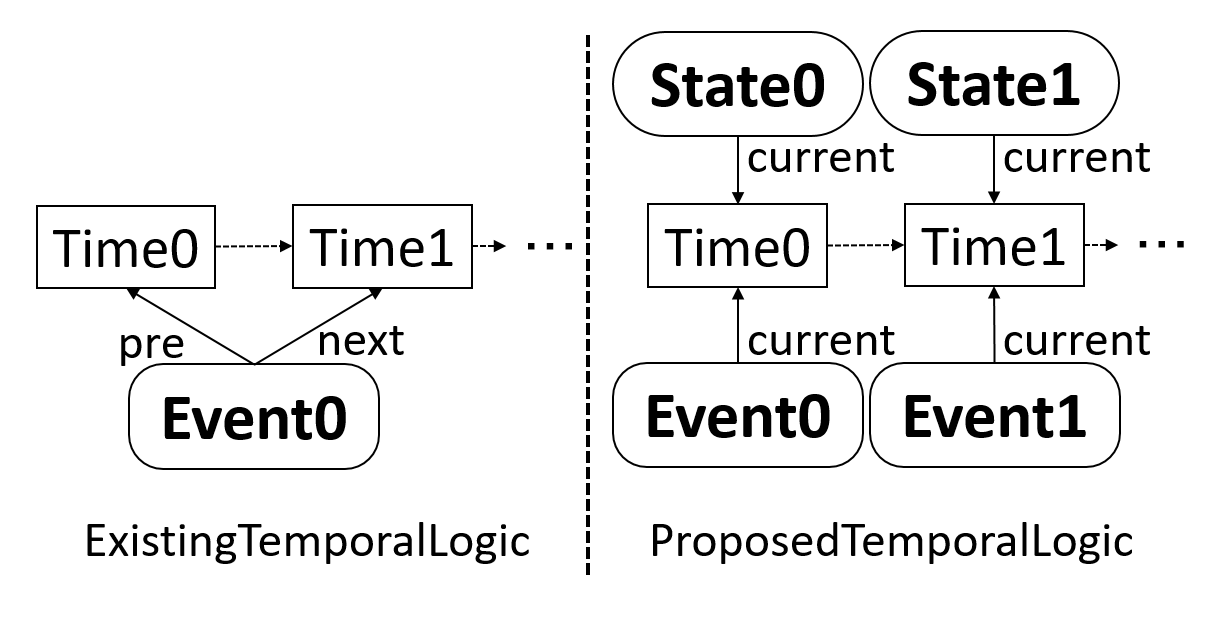
\includegraphics[width=\hsize]{./fig/TimeClass.eps}
\caption{提案モデルにおける時間軸とイベントの関係}
\label{fig:TimeClass}
\end{figure}

この表現の変更によって、二つの既存モデルそれぞれにおける時相論理の表現能力に変更はない。
そもそも基礎モデルにおいて、二つのTimeクラスのインスタンスを利用する関係性を採用した理由は今後の拡張性を想定したためである。
基礎モデルには「リクエストやレスポンスといったイベントが同時刻で発生しない」といった制限が存在しており、このようなTimeクラスの関係性を用いていた場合には、この制限を取り払う拡張が容易となると考えられていた。
しかし、表現の変更後も同様に制限を取り除く拡張は可能である。
つまり、この変更によって既存モデルの表現能力と拡張性を妨げることはない。

\subsection{汎用的な状態クラス}
\label{sec:state-class}
導入する状態クラスとしてCode\ref{code:StateClass}に示すStateクラスを定義する。
このStateクラスの要素であるflowはStateクラス同士を接続し状態の遷移を表し、currentはその状態となり得る時刻を表す。
また、その他の項目としてEqItem、DifItemクラスをStateクラスの変数としている。
\begin{lstlisting}[caption=Stateクラス, label=code:StateClass]
abstract sig State{
	flow: set State,
	eq: one EqItem,
	dif: one DifItem,
	current: set Time
}
abstract sig EqItem{}
abstract sig DifItem{}
sig StateTransaction extends HTTPTransaction{
	beforeState: set State,
	afterState: set State
}
\end{lstlisting}

まず、EqItemは同一の状態遷移上で変化しない要素(以下、「不変項目」とする)を表すクラスである。
不変項目は複数のStateが存在する場合に、いずれのStateが同一の遷移であるのかを判定するために用いる。
これは、ウェブ上には様々な要素が存在し、それらの要素が各一つずつであるとは限らないためである。
このような場合には、状態遷移が並列に混在するため、どのインスタンスが同一の遷移に属するかを判定する必要があり、不変項目はこれを可能とする。

また、DifItemは状態遷移において変化する要素(以下、「変化項目」とする)を表すクラスである。
この部分には、あるウェブの要素の状態変化を表現する上で変化しうる内容を記述する。

最後に、これらのStateはCookieモデルと同様にHTTPTransactionに関連付けることで、レスポンスとリクエスト時の状態を表すように配置する。
具体的に、HTTPTransactionを継承しStateクラスを持つStateTransactionをCode\ref{code:StateClass}の9-12行目で定義している。

このStateクラスを利用してウェブの要素の状態遷移を考えるには、State、EqItem、DifItemクラスを継承するその要素専用のクラスを定義する。
また、その要素について不変項目と変化項目を明らかにしておき、継承後のクラスに記述する。
以下のCode\ref{code:CookieClass}はCookieモデルを基にしたCookieへの応用例である。
2,3行目に記すように、Stateを継承するクラスではeqとdifもまた、EqItem、DifItemを継承する専用のクラスに含まれるように条件を記述する。
Cookieモデルでは、不変項目がクライアント、変化項目がCookieの集合となっている。
これは、各クライアント毎にCookieの保存が行われているため、状態遷移の上でクライアントは変更されないためである。
また、変化項目は状態遷移で変化しうる要素、つまり、クライアント内で保存されているCookieを表現する。
\begin{lstlisting}[caption=Cookieへの応用例, label=code:CookieClass]
sig CookieState extends State{}{
	eq in CookieEqItem
	dif in CookieDifItem
}
sig CookieEqItem extends EqItem{
	client: one HTTPClient
}
sig CookieDifItem extends DifItem{
	cookie: set Cookie
}
\end{lstlisting}

\subsection{直前の状態を判定する述語}
\ref{sec:state-class}で述べたStateクラスに対して、同一の状態遷移上で直前となる状態を判定する述語LastStateを利用できる。
このLastStateは三つの引数を要し、そのうちの二つはStateでありそれぞれpre、postと表す。
ここで、述語LastStateはpreがpostの直前の状態である場合に真となるよう作成する。
しかし、postが複数の時刻で継続している状態である場合にはpostは複数の時刻を持つ。
したがって、この二つの入力のみでは一つのpostに対して真となるpreが複数存在することになる。
これを防ぐために、postの時刻を指定するStateTransactionを引数に追加する(これをstrとする)。
これにより、与えられたトランザクションに含まれるpostの時刻に限定して、その時刻においてpreが直前であるか判定でき、真となる組み合わせが一意に定まる。
このように作成した述語LastStateをCode\ref{code:LastState}に示す。

\begin{lstlisting}[caption=状態遷移において直前の状態を判定する述語, label=code:LastState]
pred LastState[pre:State, post:State, str:StateTransaction]{
	pre.eq = post.eq
	post in str.(beforeState + afterState)

	some t,t':Time |
		{
			t in pre.current
			t' in str.(request + response + re_res).current
			t' in str.request.current implies post in str.beforeState
			t' in str.(response + re_res).current implies post in str.afterState
			t' in t.next.*next

			all s:State, t'':Time |
				(s.eq = pre.eq and t'' in s.current) implies
						(t in t''.*next) or (t'' in t'.*next)
		}
}
\end{lstlisting}

また、述語LastStateが真となる条件は以下のように整理できる。
\begin{itembox}[l]{LastState}
LastStateは引数pre,post(Stateクラス), str(StateTransactionクラス)が以下をすべて満たす場合に真となる。
\begin{itemize}
\item preとpostの不変項目が同一である
\item postがstrのbeforeState、afterStateのいずれかに属している
\item preの時刻とpostのstrにおける時刻の間の時刻を持つ、不変項目が同一の他の状態が存在しない
\end{itemize}
\end{itembox}

\subsection{初期状態を判定する述語}
Stateクラスに対して利用可能な、もう一方の述語は初期状態を判定する述語InitialStateである(Code\ref{code:InitialState}参照)。
引数としてStateクラスが与えられ(これをsとする)、それが初期状態であるか判定する。
また、不変項目が異なると状態変化がそれぞれ独立するため、それぞれに対して初期状態が生じる(図\ref{fig:InitialState})。
\begin{lstlisting}[caption=状態遷移において初期状態を判定する述語, label=code:InitialState]
pred InitialState[s:State]{
	all s':State |
		s.eq = s'.eq implies
			s'.current in s.current.*next
}
\end{lstlisting}

\begin{itembox}[l]{InitialState}
InitialStateは引数s(Stateクラス)に対して、sと同じ不変要素を持つStateクラスのインスタンスがすべてsの時刻以降の状態である場合に真となる
\end{itembox}

\end{document}
